% --------------------------------------------------
% 
% This chapter is for dingo
% 
% --------------------------------------------------

\chapter{Software development to establish metabolic flux sampling 
         approaches at the community level}
\label{cha:dingo}

% ADD AN INTRO FOR THE SECTION


% The relationship between genotype and phenotype is fundamental to biology.
% Many levels of control are introduced when moving from one to the other. 
% Systems biology aims at deciphering "the strategy" both at the cell and at higher levels of organization, in case of multicell species, that enables organisms to produce orderly adaptive behavior in the face of widely varying genetic and environmental conditions (\cite{strohman2002maneuvering}); the term "strategy" is used as per \cite{polanyi1968life}.
% Systems biology approaches aim at interpreting how a system's properties emerge; from the cell to the community level.


\section{A New MCMC Algorithm for Sampling the Flux Space of
Metabolic Networks}

   Publication relative to this chapter: \cite{chalki2021SoCG}

\subsection{Introduction}


   Systems Biology is a fundamental field and paradigm that represents a crucial era in Biology. 
   Its functionality and usefulness rely on metabolic networks that model the reactions occurring inside an organism and provide the means to understand the underlying mechanisms that govern biological systems. 
   We address the problem of sampling uniformly steady states of a metabolic network. 
   We use a convex polytope to represent this set. 
   However, the polytopes that result from biological data are of very high dimension (in the order of thousands) and in most, if not all, the cases are considerably skinny. 
   Therefore, to perform uniform sampling efficiently in this setting, we need a novel algorithmic and computational framework specially tailored for the properties of metabolic networks. 
   We present a complete software framework to handle sampling from convex polytopes that result from metabolic networks. 
   Its backbone is a Multiphase Monte Carlo Sampling (MMCS) algorithm.
   We demonstrate the efficiency of our approach by performing extensive experiments on various metabolic networks. 
   Notably, sampling on the most complicated human metabolic network accessible today, Recon3D, corresponding to a polytope of dimension $5\,335$, took less than $30$ hours. 
   To the best of our knowledge, that is out of reach for existing software.

   \begin{figure}[!htbp]
      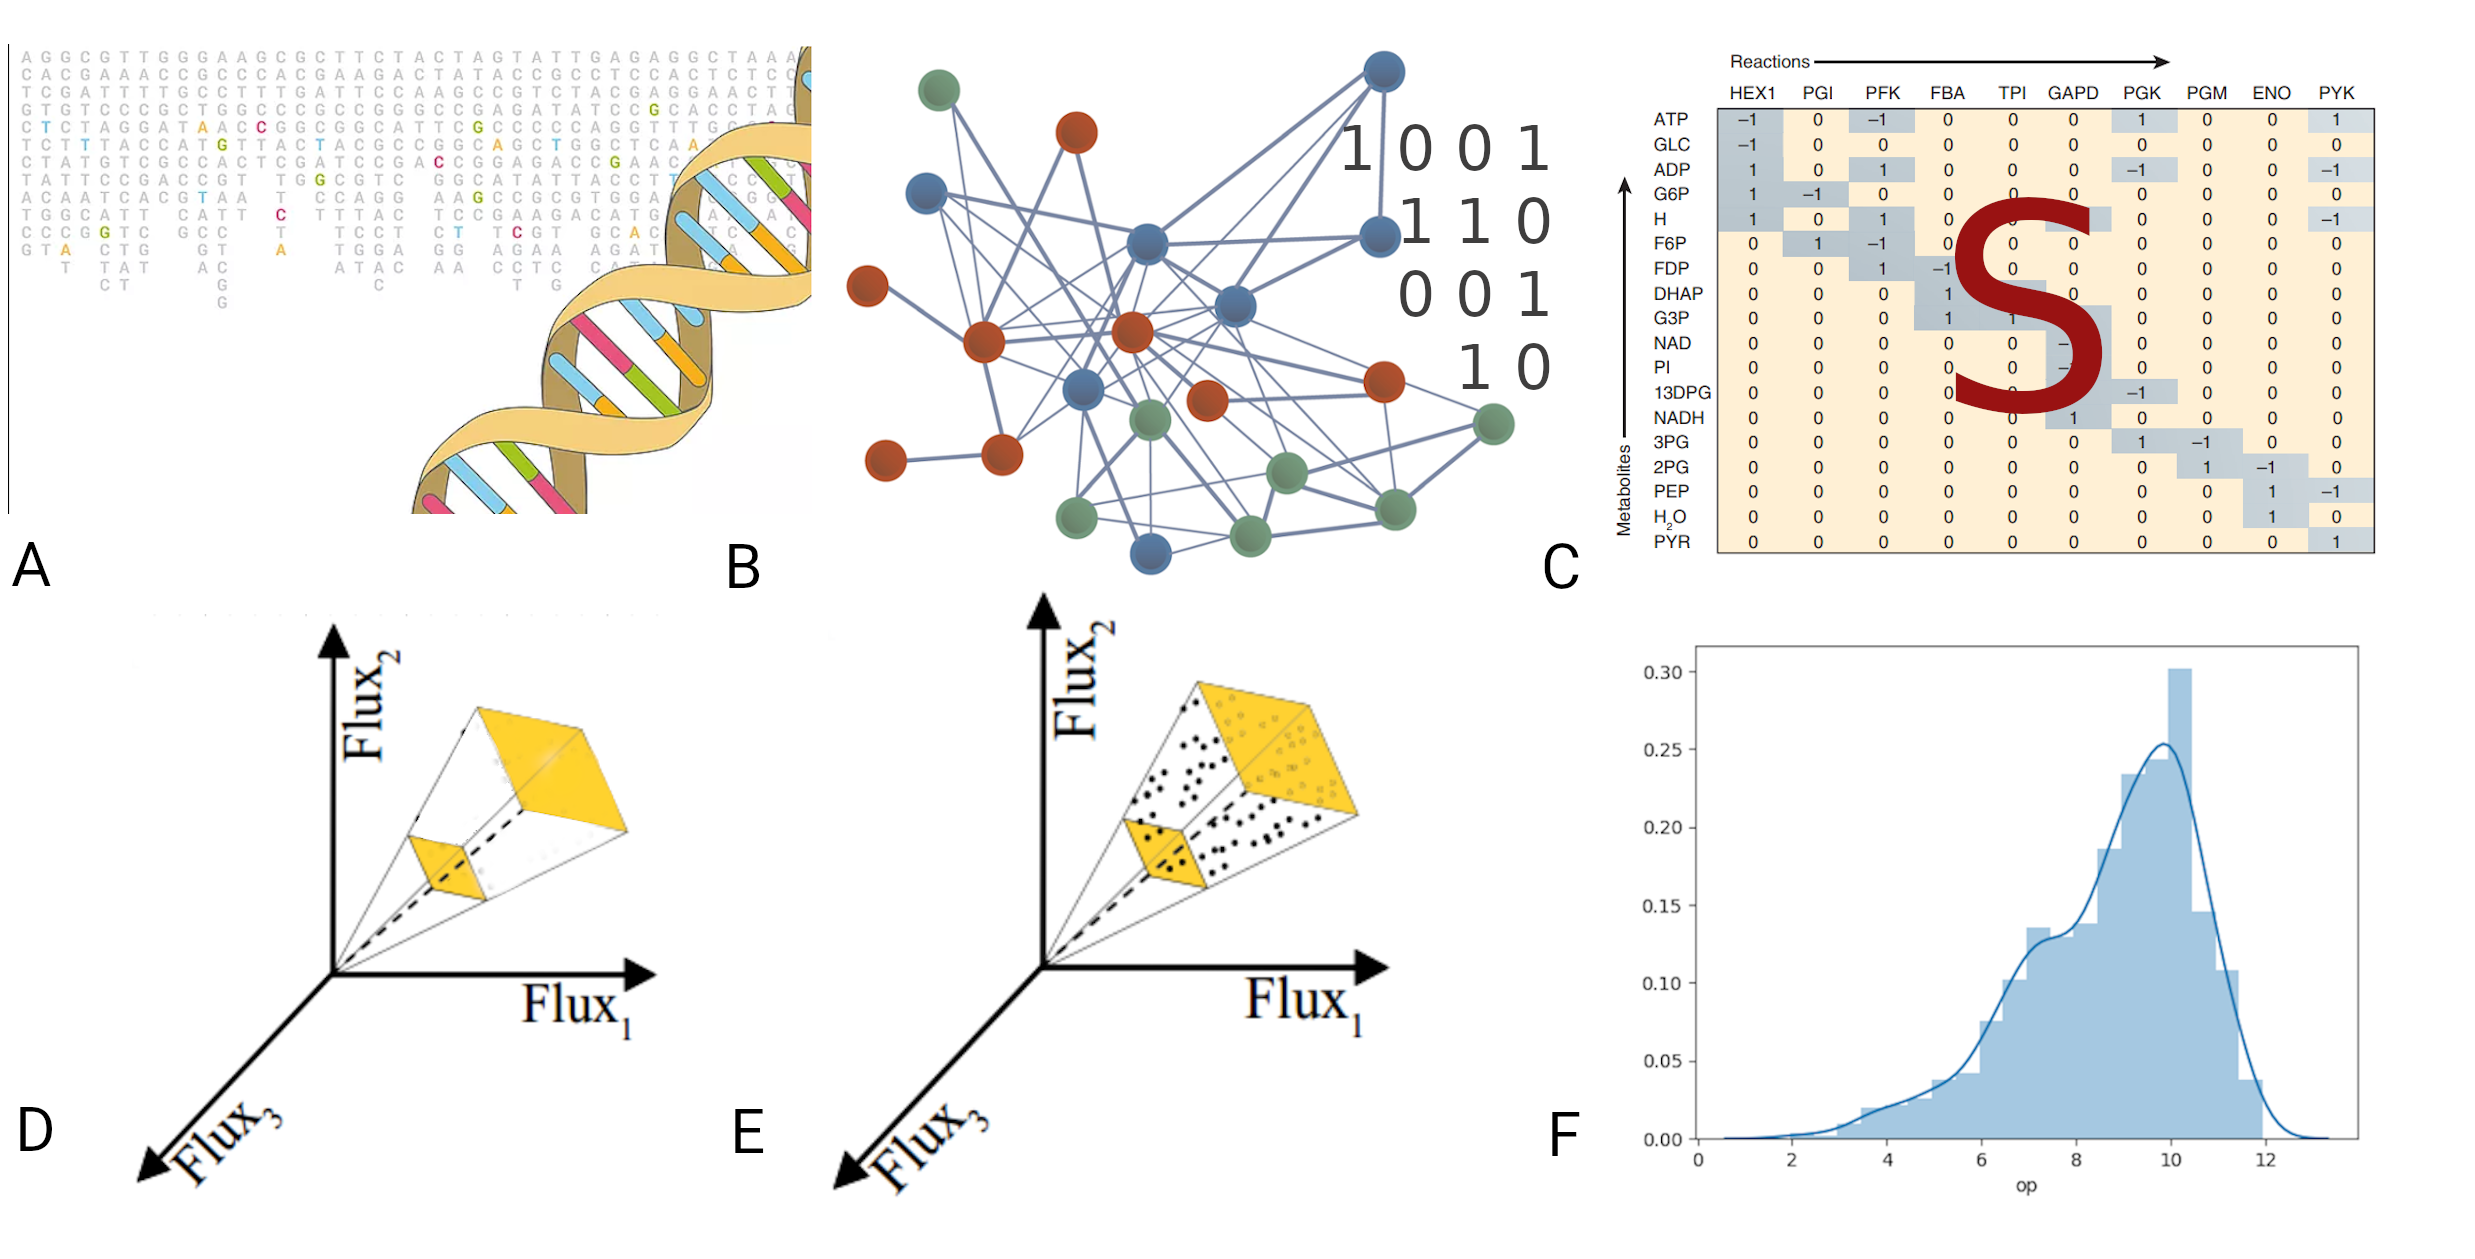
\includegraphics[width=1.0\columnwidth]{figures/flux_sampling_workflow.png}
      \caption{
         From DNA sequences to distributions of metabolic fluxes.
         (A) The genes of an organism provide us with the enzymes that it can potentially produce. Enzymes are like a blueprint for the reactions they can catalyze.
         (B) Using the enzymes we identify the reactions in the organism.
         (C) We construct the stoichiometric matrix of the metabolic  model.
         (D) We consider the flux space under different conditions (e.g., steady states);
         they correspond  to  polytopes containing flux vectors addressing these conditions.
         (E) We sample from polytopes that are typically skinny and of high dimension.
         (F) The distribution of the flux of a reaction provides  great insights
         to biologists.
      }
      \label{fig:sampling_workflow}
   \end{figure}

   But why being interested in such a task ? The genome of most bacteria are rather short to have issues like that. 

   However, MAGs can be brought together and build the metabolic model of a whole community! 



   \begin{figure}[h]
      \centering
      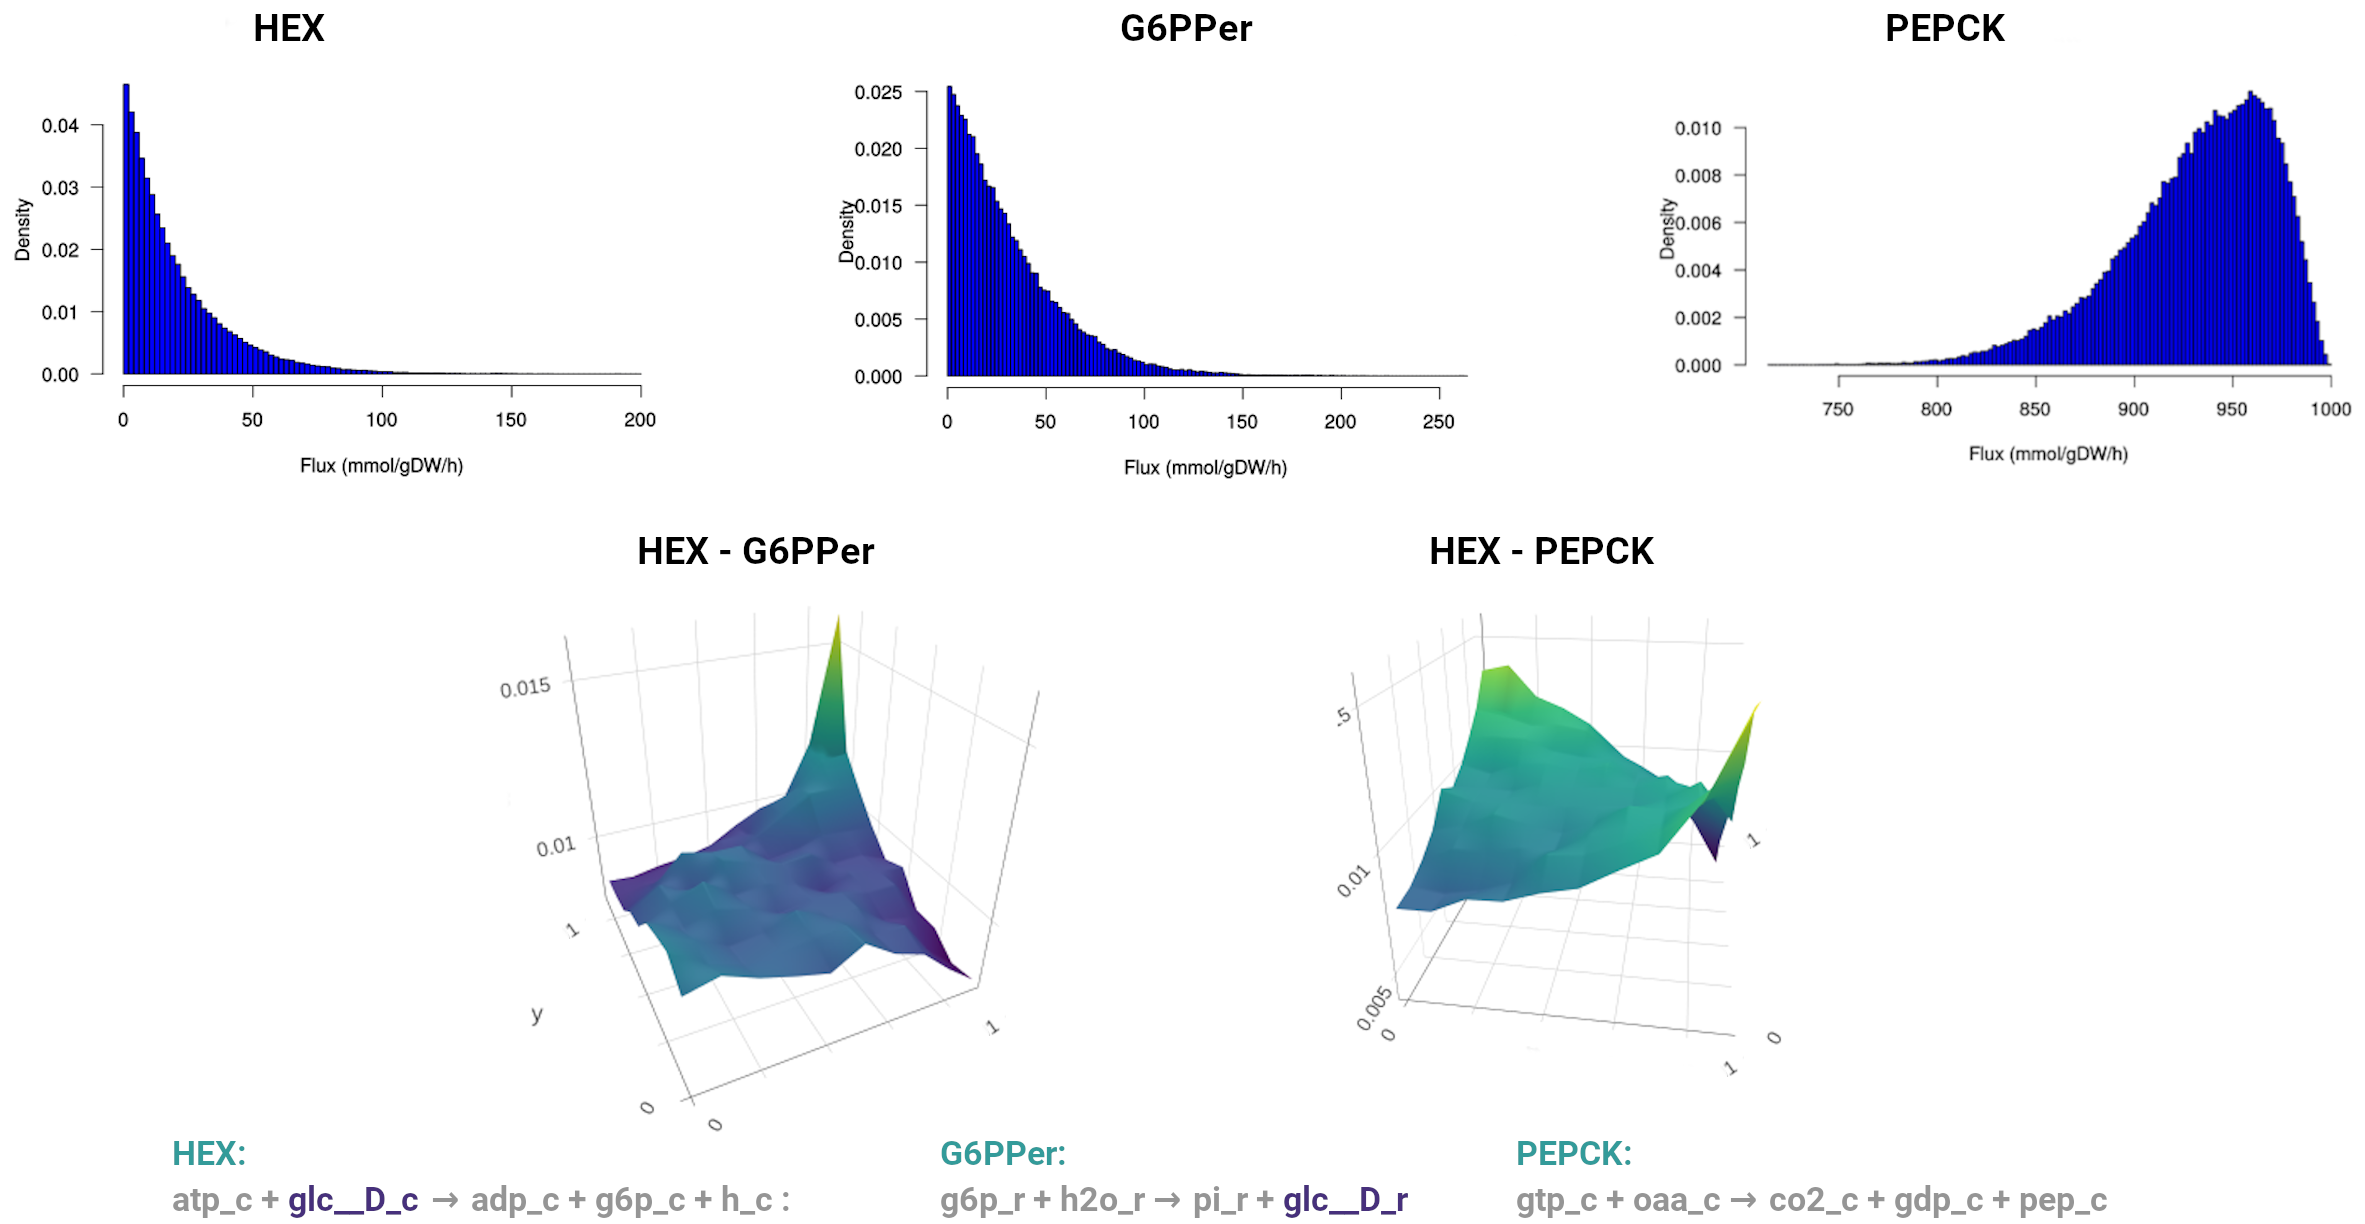
\includegraphics[width=125mm]{figures/copulas_cropped.png}
      \caption{
         Flux distributions in the most recent human metabolic network Recon3D~\cite{brunk2018recon3d}. 
         We estimate the flux distributions of the reactions catalyzed by the enzymes Hexokinase (D-Glucose:ATP) (HEX), Glucose-6-Phosphate Phosphatase, Edoplasmic Reticular (G6PPer)
         and Phosphoenolpyruvate carboxykinase (GTP) (PEPCK).
         As we sample steady states, the production rate of $glc\_\_D \_c$ should be equal to its consumption rate. 
         Thus, in the corresponding copula, we see a positive dependency between HEX,
         i.e., the reaction that consumes $glc\_\_D \_c$ and G6PPer, that produces it.
         Furthermore, the PEPCK reaction operates when there is no $glc\_\_D\_c$ available and does not operate when the latter is present.
         Thus, in their copula we observe a negative dependency between HEX and PEPCK.
         A copula is a bivariate probability distribution for which the marginal probability distribution of each variable is uniform.
         It implies a positive dependency when the mass of the distribution concentrates along the up-diagonal (HEX - G6PPer)
         and a negative dependency when the mass is concentrated along the down-diagonal (HEX - PEPCK). %~\cite{Cales18}.
         The bottom line contains the  reactions and their stoichiometry.
      }
   \end{figure}




\subsection{Methods}


\subsubsection{Efficient Billiard walk}

   \begin{figure}[h]
      \centering
      \textbf{Algorithm 1: }Billiard Walk$(P, p, \rho, \tau, W)$
      \medskip
      \label{alg:billiard}

      \begin{algorithmic}
         \REQUIRE polytope $P$; point $p \in P$; upper bound on the number of reflections
         $\rho$; \\ parameter $\tau$ to adjust the length of the trajectory; walk length $W$.
         \ENSURE a point in $P$ (uniformly distributed in $P$).
         \FOR {$j=1,\dots ,W$} 
         \STATE {
            $L \leftarrow -\tau\ln\eta$;  $\ \eta\sim \mathcal{U}(0,1) \quad$ \COMMENT{
               {\textit{length of the trajectory}}
               }
            $i\leftarrow 0 \quad $ \COMMENT{
               {\textit{current number of reflections}}
               }
            $p_0\leftarrow p \quad $ \COMMENT{
               {\textit{initial point of the step}}
               }
            pick a uniform vector $u_0$ from the unit sphere
            \COMMENT{
               {\textit{initial direction}}}
         }
         \WHILE{$i\leq \rho$}
         \STATE{$\ell \leftarrow \{p_i + tu_i, 0\leq t\leq L\} \quad$} \COMMENT{
            {\textit{this is a segment}}}

         \IF{$\partial P \cap \ell = \O$} 
            \STATE{$p_{i+1} \leftarrow p_i+Lu_i \quad$
                  \textbf{break} \;}
         \ENDIF
         
         \STATE{$p_{i+1} \leftarrow \partial P\cap\ell ; \quad$}
         \COMMENT{
            {\textit{point update}}
            }
            
         \STATE{the inner vector, $s$, of the tangent plane at $p$, \\
            \ \ s.t.\ $||s|| = 1$,\; $L \leftarrow L - |P\cap\ell|$,
         $u_{i+1} \leftarrow u_i - 2(u_i^Ts) s \quad$}
         \COMMENT{
            {\textit{direction update}}
            }

         \STATE{$i \leftarrow i+1$}

         \ENDWHILE
      
         \IF{$i=\rho$}
            \STATE{$p \leftarrow p_0$}
         \ELSE	
            \STATE{$p \leftarrow p_i$}
         \ENDIF
         

         \ENDFOR

      \RETURN $p$\;


      \end{algorithmic}
         
   \end{figure}

   At each step of Billiard Walk, we compute the intersection point of a ray, say
   $\ell:=\{p+tu,\ t\in\mathbb{R}_+ \}$,
   with the boundary of $P$, $\partial P$, and the normal vector of the tangent
   plane of $P$ at the intersection point.
   The inner vector of the facet that the intersection  point belongs to is a row of $A$.
   To compute the point $\partial P\cap\ell$ where the first reflection of a Billiard Walk
   step takes place we need to compute the intersection of $\ell$ with all the hyperplanes that define the facets of $P$.
   This corresponds to solve (independently) the following $m$ linear equations
   \begin{equation}
     a_j^T(p_0 + t_ju_0) = b_j \Rightarrow t_j = (b_j - a_j^Tp_0) / a_j^Tu_0,\ j \in[k],
   \end{equation}
   and keep the smallest positive $t_j$; $a_j$ is the $j$-th row of the matrix $A$.
   We solve each equation in $\mathcal{O}(d)$ operations and so the overall complexity is
   $\mathcal{O}(d k)$, where $k$ is the number of rows of $A$ and thus an upper bound on
   the number of facets of $P$. A straightforward approach for Billiard Walk would
   consider that each reflection costs $\mathcal{O}(k d)$ and thus the per step cost is
   $\mathcal{O}(\rho kd)$. However, our improved version performs more efficiently both
   \textit{point} and \textit{direction updates} in pseudo-code by storing some
   computations from the previous iteration combined with a preprocessing step. The
   preprocessing step involves the normal vectors of the facets and takes $k^2 d$
   operations. So the amortized per-step complexity of Billiard Walk becomes
   $\mathcal{O}((\rho + d)k)$. The pseudo-code appear in Algorithm~\ref{alg:billiard}.
   
   
   
   % lemma 
   % \begin{lem}
   %     \label{lem:BW-step-cost}
   %     The amortized cost per step complexity of Billiard Walk
   %     (Algorithm~\ref{alg:billiard}) is $O((\rho + d)k)$ 
   %     after a preprocessing step that takes $O(k^2d)$ operations, where $\rho$ is the maximum number of reflections per step.
   %  \end{lem}



   \subsubsection{Multiphase Monte Carlo Sampling algorithm}

   \begin{figure}[!htbp]
      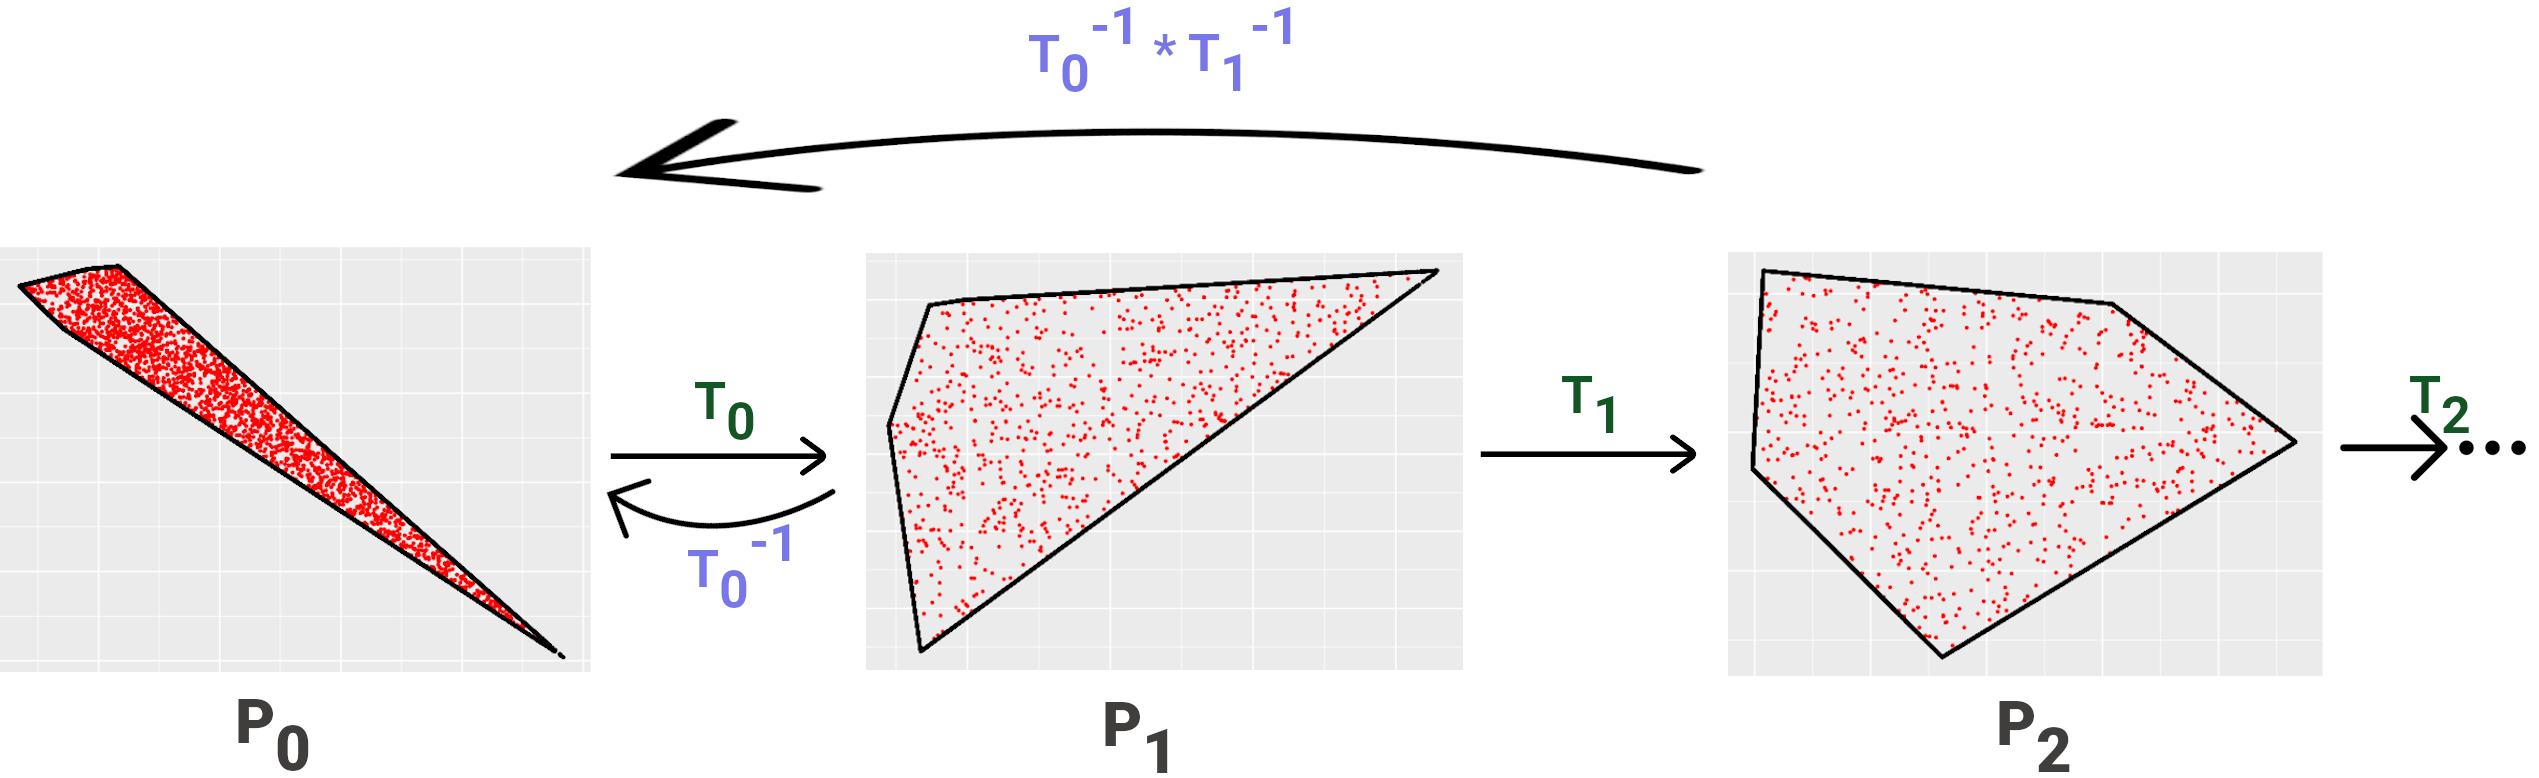
\includegraphics[width=1.0\columnwidth]{figures/sampling_extra_phase_croped.png}
      \caption{
         An illustration of our Multiphase Monte Carlo Sampling algorithm. The method is given an integer $n$ and starts at phase $i=0$ sampling from $P_0$. In each phase it samples a maximum number of points $\lambda$. If the sum of Effective Sample Size in each phase becomes larger than $n$ before the total number of samples in $P_i$ reaches $\lambda$ then the algorithm terminates. Otherwise, we proceed to a  new phase.
    We map back to $P_0$ all the generated samples of each phase.
      }
      \label{fig:mmcs}
   \end{figure}


\subsection{Results}


\subsection{Discussion}

   Flux sampling at the community level!


% From \citet{price2004genome} :
% "Pairwise correlation coefficients can be calculated
% between all reaction fluxes based on uniform random
% sampling. Perfectly correlated reactions (R2 = 1) operate
% as functional modules within a biochemical network,
% whereas uncorrelated reactions (R2 ~0) operate independently of each other. The degree of independence
% between reactions is an important consideration when
% choosing a set of fluxes to measure that will best determine the operating state of a biochemical network"


% Write something from \citeauthor{polanyi1968life}

% \section{The `dingo` Python library}






